\documentclass[11pt,a4paper]{article}   	
\usepackage[utf8]{inputenc}              	
\usepackage[czech]{babel}                	
\usepackage[pdftex]{graphicx}
\usepackage{amsfonts}				
\begin{document}
\section{Mapování vazeb}
	\subsection{Úvod - upřesnění formulace}
	Zkratka $OC$ (Ordering Column) značí sloupec, určující pořadí prvků, tedy vlastnost property isOrdered. \\
	$FK[B]$ značí cizí klíč ze třídy B.
		\begin{figure}	             
    		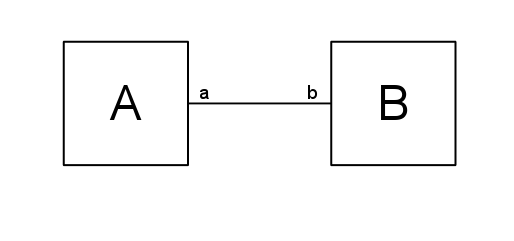
\includegraphics[scale=0.9]{./AB.png}
    		\caption{Pro lepší představu obrázek vazby}			     
    		\label{pict:vazba}		             
   		\end{figure}
	\subsection{Obecné guardy}
	     \begin{itemize}
	     	\item $ g_0 $\texttt : {Pouze obyčejná vazba}				
         	\item $ g_1 $\texttt : {isOpposite = TRUE}
         	\item $ g_2 $\texttt : {isCollection = TRUE}
         	\item $ g_3 $\texttt : {isCollection = TRUE $\wedge$ isOpposite = TRUE}
         	\item $ g_4 $\texttt : {isCollection = TRUE $\wedge$ isOrdered = TRUE}    		  							
   		\end{itemize}						                                
	\subsection{Vlastnosti mapované na prázdnou množinu}
   		Jedná se o dvě základní vlastnosti tříd. Pokud je třída 
   		Transient namapuje se její property na prázdnou množinu. 
   		\begin{itemize}				    
         	\item \texttt	{
         					$\pi_0(b) : E \to \{ 0\}$  
         					}
   		\end{itemize}
   		Pokud je třída Embadded, namapují se její sloupce do třídy, která třídu využívá.
   	\subsection{Jednostranně navigabilní vazby}
   		Třída A vidí skrz svoji property na trídu B, ale B nemá žádnou takovou property a 
   		tak třídu A nevidí a ani neví, že je třídou A viděna. Při jednostranně navigabilním
   		mapování sice třída B třídu A nevidí, ale v databázi na ni má uloženy FK.
   		\\
   		Máme dva případy mapování:
   		\begin{itemize}				    
         	\item 			$ \omega(\pi_1,g_3)$\\
         					$\pi_1(b) : E \to \{ sloupec, OC\}$
         					
         	\item         	$\omega(\pi_2, g_3 \vee g_2)$ \\
         					$\pi_2(b) : E \to \{ sloupec\}$
         	\item Jako třetí případ můžeme považovat $g_0$. Tento případ je ale stejný, 
         	jako u případů oboustranně navigabilních, tak bude mezi nimi.	  							
   		\end{itemize}
   	\subsection{Oboustranně navigabilní vazby}
   		Třída A vidí skrz svoji property na třídu B a třída vidí skrz svou property na třídu A. \\
   		Máme sedm případů mapování, které je asi nejlepší rozdělit podle toho, zda je $g_1$ kolekce, či ne.
   		\subsubsection{b.isOpposite}
   		V tomto případě máme obecně už jen dva možné výstupy:
   		   		\begin{itemize}				    
         			\item 
         							$\omega(\pi_3(b), g_0 \vee g_1) \wedge \omega(\pi_3(a), g_2 \vee g_3)$\\
         							$\pi_3(b) : E \to \{ sloupec, FK[A]\}$ \\
         							$\pi_3(a) : E \to \{ 0\}$
         			\item 			$\omega(\pi_4(b), g_1) \wedge \omega(\pi_4(a), g_4)$\\
         							$\pi_4(b) : E \to \{ sloupec, OC, FK[A]\}$ \\
         							$\pi_4(a) : E \to \{ 0\}$  		  							
   				\end{itemize}
   		\subsubsection{b.isOpposite.isCollection}
   		Tato část je poměrně obsáhlá, ale ve finále vede pouze na pět různých mapování:
   				\begin{itemize}				    
         			\item			$\omega(\pi_5(b),g_1 \wedge g_4) \wedge \omega(\pi_5(a), g_0)$\\        							
         							$\pi_5(b) : E \to \{ sloupec, OC\}$ \\
         							$\pi_5(a) : E \to \{ sloupec, FK[B]\}$		
         			\item			$\omega(\pi_5(b),g_1 \wedge g_4) \wedge \omega(\pi_5(a), g_4)$\\    							
         							$\pi_6(b) : E \to \{ sloupec, OC\}$ \\
         							$\pi_6(a) : E \to \{ sloupec, OC\}$	\\	
         							(Vznik vazební tabulky s cizími klíči)
         			\item			$\omega(\pi_5(b),g_1 \wedge (g_3 \vee g_2)) \wedge \omega(\pi_5(a), g_0)$\\   							
         							$\pi_7(b) : E \to \{ 0\}$ \\
         							$\pi_7(a) : E \to \{ sloupec, FK[B]\}$	\\
         			\item			$\omega(\pi_5(b),g_1 \wedge g_3) \wedge \omega(\pi_5(a), g_4)$\\
         							$\omega(\pi_5(b),g_1 \wedge g_2) \wedge \omega(\pi_5(a), g_4)$\\
         							$\omega(\pi_5(b),g_1 \wedge g_4) \wedge \omega(\pi_5(a), g_3)$\\
         							$\omega(\pi_5(b),g_1 \wedge g_4) \wedge \omega(\pi_5(a), g_2)$\\             							
         							$\pi_8(b) : E \to \{ 0\}$ \\
         							$\pi_8(a) : E \to \{ sloupec, OC\}$	\\	
         							(Vznik vazební tabulky s cizími klíči)	 
         		     \item 			$\omega(\pi_5(b),g_1 \wedge g_3) \wedge \omega(\pi_5(a), g_3)$\\
         							$\omega(\pi_5(b),g_1 \wedge g_3) \wedge \omega(\pi_5(a), g_2)$\\
         							$\omega(\pi_5(b),g_1 \wedge g_2) \wedge \omega(\pi_5(a), g_3)$\\
         							$\omega(\pi_5(b),g_1 \wedge g_2) \wedge \omega(\pi_5(a), g_2)$\\       							
         							$\pi_9(b) : E \to \{ 0\}$ \\
         							$\pi_9(a) : E \to \{ 0\}$	\\	
         							(Vznik vazební tabulky s cizími klíči)	 				   							
   				\end{itemize}			   		    
\end{document} %konec dokumentu